% http://www.ctan.org/tex-archive/macros/latex/contrib/beamer/examples
% http://latex.artikel-namsu.de/english/beamer-examples.html

%\documentclass{beamer}
\documentclass[usenames,dvipsnames]{beamer}
\usepackage{amsmath}
\usepackage{amssymb}
\usepackage{bm}
\usepackage{fancybox, graphicx}
\usepackage{listings}
\usepackage{tikz} % Diagrams
\usepackage{color}
\usepackage{textcomp} % See https://tex.stackexchange.com/questions/145416/how-to-have-straight-single-quotes-in-lstlistings

\lstset{language=bash,upquote=true} % Format listings as appropriate for bash. Inexplicably we get problems if the language is set as part of the \begin{lstlisting} command.

% https://tex.stackexchange.com/questions/36030/how-to-make-a-single-word-look-as-some-code
\definecolor{light-gray}{gray}{0.95}
\newcommand{\code}[1]{\colorbox{light-gray}{\texttt{#1}}}



\usetheme{boxes}
\usecolortheme{beaver}


\title{Introduction to git}

\author{Lorne Whiteway \\ lorne.whiteway@star.ucl.ac.uk}

\institute[UCL]
{
  Astrophysics Group\\
  Department of Physics and Astronomy\\
  University College London
}
\date
{17 November 2017}

\subject{IT}

\begin{document}

\frame{\titlepage}

\begin{frame}{Where to find this presentation}
  \begin{block}{}
    Find the presentation at \alert{\url{https://tinyurl.com/y8pr4mvq}}.\\
  \end{block}
  \begin{block}{}
    On this page click on `Download' to get a copy of the presentation.
  \end{block}
\end{frame}

\begin{frame}{\url{https://xkcd.com/1597/} {\tiny Creative Commons Attribution-NonCommercial 2.5 License.}}
  \begin{block}{}
    \begin{center}
      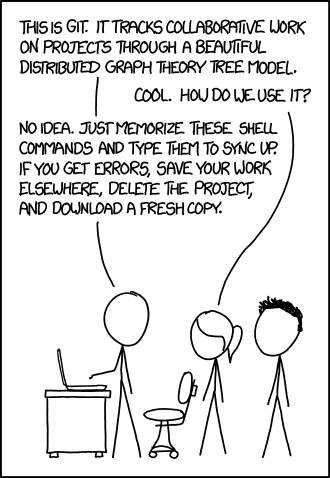
\includegraphics[scale=0.45]{xkcd_1597.png}
    \end{center}
  \end{block}
\end{frame}

\begin{frame}{Some commentary...}
  \begin{block}{}
    \url{https://stevebennett.me/2012/02/24/10-things-i-hate-about-git/}
  \end{block}
\end{frame}

\begin{frame}{Purpose of presentation}
  \begin{block}{}
    \begin{itemize}
      \item{I don't want to teach you how to use git.}
      \item{Rather I want to illustrate (part of) git's `internal model' and to define certain key git terminology so that you will be better prepared to teach yourself git.}
      \item{My examples assume you are calling git from the command-line. Friendlier interfaces to git exist - but you still need to know the underlying model to use them effectively.}
    \end{itemize}
  \end{block}
\end{frame}


\begin{frame}{Why is git (relatively) hard to come to terms with?}
  \begin{block}{}
    \begin{itemize}
      \item{The internal model is complicated.}
      \item{The interface is inconsistent.}
      \item{The documentation is suboptimal.}
      \item{Several key ideas have been given misleading names.}
      \item{It uses a `distributed' model whereas what you usually want is a `client/server' model. So you tend to be `fighting against the paradigm'...}
    \end{itemize}
  \end{block}
\end{frame}

\begin{frame}{Source control}
  \begin{block}{}
    \begin{itemize}
      \item{Source control is software to `keep track of' (i.e. store) successive versions as we edit a collection of \textit{source} files (computer code, \LaTeX{} documents, etc.)}
      \item{Works best if the source is text, not binary. Intermediate files are usually not kept track of. Output files might be - your choice.}
      \item{Any serious project should be under source control.}
    \end{itemize}
  \end{block}
\end{frame}


\begin{frame}{Working directory and repository}
  \begin{block}{}
    \begin{itemize}
      \item{You need a \textit{working directory} and a \textit{repository}.}
      \item{The working directory and its subdirectories contain the actual files that you are editing.}
      \item{The repository is some sort of database containing all previous versions.}
      \item{One model would be to put the repository on the Internet or Intranet where everyone can see it...}
    \end{itemize}
  \end{block}
\end{frame}

\begin{frame}{Location of git repositiory}
  \begin{block}{}
    \begin{itemize}
      \item{... But in git the repository is \textbf{next to} the working directory, in a hidden subdirectory (called .git) of the top-level working directory.}
    \end{itemize}
    \begin{center}
      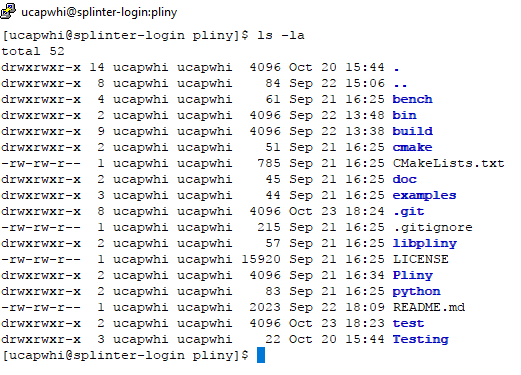
\includegraphics[scale=0.5]{ls_output.png}
    \end{center}
  \end{block}
\end{frame}

\begin{frame}{This has consequences...}
  \begin{block}{}
    \begin{itemize}
      \item{You therefore need to have a git repository next to your working directory on your local directory (where you are doing the actual editing).}
      \item{But typically you will also need one on the internet (for backup and for collaboration and sharing).}
      \item{So you will typically be dealing with \textbf{two} git repositories (and dealing with the issues of keeping them in synch.}
    \end{itemize}
    \begin{itemize}
      \item{The upside is that you can still do version control even if you are not connected to the Internet.}
    \end{itemize}
  \end{block}
\end{frame}

\begin{frame}{Example repository content}
  \begin{figure}
    \begin{center}
      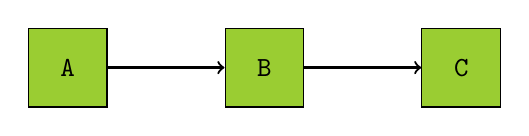
\begin{tikzpicture}[font=\ttfamily]
        \node (A) at (-2.5,5) [rectangle, draw,minimum height=1cm, minimum width=1cm, align=center, fill=YellowGreen] {A};
        \node (B) at (0.0,5) [rectangle, draw,minimum height=1cm, minimum width=1cm, align=center, fill=YellowGreen] {B};
        \node (C) at (2.5,5) [rectangle, draw,minimum height=1cm, minimum width=1cm, align=center, fill=YellowGreen] {C};
        \draw [->,thick] (A.east) -- (B.west) node [midway,left] {};
        \draw [->,thick] (B.east) -- (C.west) node [midway,left] {};
      \end{tikzpicture}
    \end{center}
  \end{figure}
  \begin{block}{}
    \begin{itemize}
      \item{This repository contains three successive versions of the files in the working directory (and its subdirectories).}
      \item{Each version is represented here as a \textit{node} (in green).}
      \item{An initial set of files (version A) was comitted to the repository; the files were then edited and the new file set (version B) was comitted; the files were then edited and comitted a third time (version C).}
    \end{itemize}
  \end{block}
\end{frame}

\begin{frame}{Another example}
  \begin{figure}
    \begin{center}
      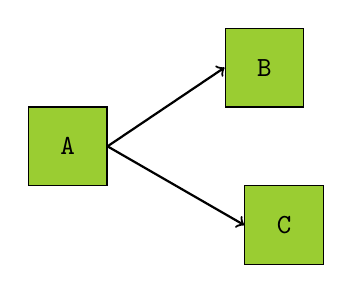
\begin{tikzpicture}[font=\ttfamily]
        \node (A) at (-1.25,5) [rectangle, draw,minimum height=1cm, minimum width=1cm, align=center, fill=YellowGreen] {A};
        \node (B) at (1.25,6) [rectangle, draw,minimum height=1cm, minimum width=1cm, align=center, fill=YellowGreen] {B};
        \node (C) at (1.5,4) [rectangle, draw,minimum height=1cm, minimum width=1cm, align=center, fill=YellowGreen] {C};
        \draw [->,thick] (A.east) -- (B.west) node [midway,left] {};
        \draw [->,thick] (A.east) -- (C.west) node [midway,left] {};
      \end{tikzpicture}
    \end{center}
  \end{figure}
  \begin{block}{}
    \begin{itemize}
      \item{Here we committed A...}
      \item{Then we edited A (to form B) and committed B...}
      \item{Then we went back to A, made a perhaps different set of edits (to form C) and committed C.}
    \end{itemize}
  \end{block}
\end{frame}

\begin{frame}{What do the arrows actually stand for?}
  \begin{figure}
    \begin{center}
      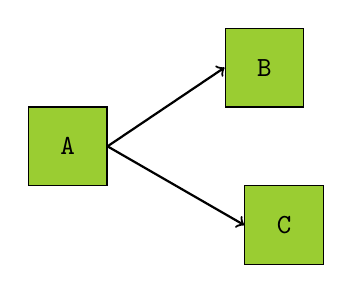
\begin{tikzpicture}[font=\ttfamily]
        \node (A) at (-1.25,5) [rectangle, draw,minimum height=1cm, minimum width=1cm, align=center, fill=YellowGreen] {A};
        \node (B) at (1.25,6) [rectangle, draw,minimum height=1cm, minimum width=1cm, align=center, fill=YellowGreen] {B};
        \node (C) at (1.5,4) [rectangle, draw,minimum height=1cm, minimum width=1cm, align=center, fill=YellowGreen] {C};
        \draw [->,thick] (A.east) -- (B.west) node [midway,left] {};
        \draw [->,thick] (A.east) -- (C.west) node [midway,left] {};
      \end{tikzpicture}
    \end{center}
  \end{figure}
  \begin{block}{}
    \begin{itemize}
      \item{An arrow respects time (pointing from an earlier version to a later version), and indicates that a node was derived from an earlier node by editing.}
      \item{Q: There exists a set of edits that would take you from B to C, so why not show that arrow as well? A: It's an \textit{itinerary} (showing the route we took), not a \textit{map} of all possible routes.}
    \end{itemize}
  \end{block}
\end{frame}

\begin{frame}{Merging}
  \begin{figure}
    \begin{center}
      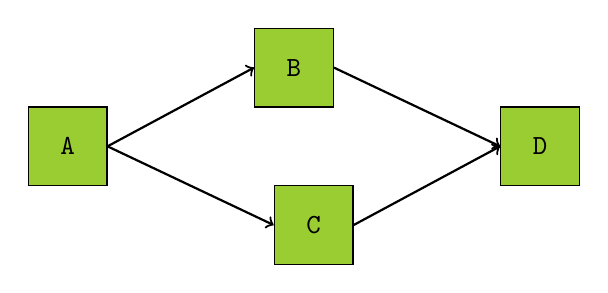
\begin{tikzpicture}[font=\ttfamily]
        \node (A) at (-3,5) [rectangle, draw,minimum height=1cm, minimum width=1cm, align=center, fill=YellowGreen] {A};
        \node (B) at (-0.125,6) [rectangle, draw,minimum height=1cm, minimum width=1cm, align=center, fill=YellowGreen] {B};
        \node (C) at (0.125,4) [rectangle, draw,minimum height=1cm, minimum width=1cm, align=center, fill=YellowGreen] {C};
        \node (D) at (3,5) [rectangle, draw,minimum height=1cm, minimum width=1cm, align=center, fill=YellowGreen] {D};
        \draw [->,thick] (A.east) -- (B.west) node [midway,left] {};
        \draw [->,thick] (A.east) -- (C.west) node [midway,left] {};
        \draw [->,thick] (B.east) -- (D.west) node [midway,left] {};
        \draw [->,thick] (C.east) -- (D.west) node [midway,left] {};
      \end{tikzpicture}
    \end{center}
  \end{figure}
  \begin{block}{}
    \begin{itemize}
      \item{Here we combined the `A to B' edits and the `A to C' edits (to form D), which was committed.}
      \item{More on such \textit{merging} later.}
    \end{itemize}
  \end{block}
\end{frame}

\begin{frame}{DAG}
  \begin{block}{}
    \begin{itemize}
      \item{Hence we get a graph (in the mathematical sense of nodes plus edges).}
      \item{The graph is not a \textit{tree} (because of merging).}
      \item{It is \textit{directed} (edges have arrows) and \textit{acyclic} (cycles would break causality), so we have a \textit{DAG} (directed acyclic graph).}
      \item{Nodes have \textit{parents} and \textit{children}, and hence \textit{ancestors} and \textit{descendents}.}
      \item{One node - the initial \textit{root} node - has no parents. All other nodes have one or two parents (or more in special cases). Thus the graph is connected, and any two nodes have ancestors in common.}
      \item{\textit{Graph theory} is an interesting part of mathematics - but alas not useful here.}
    \end{itemize}
  \end{block}
\end{frame}

\begin{frame}{Seeing the DAG}
  \begin{block}{}
    \begin{itemize}
      \item{Run \code{gitk --all} to see the DAG (lots of other information as well).}
    \end{itemize}
  \end{block}
  \begin{block}{}
    \begin{center}
      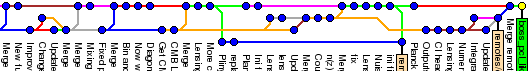
\includegraphics[scale=0.8]{DAG.png}
    \end{center}
  \end{block}
\end{frame}


\begin{frame}{What's in a node?}
  \begin{block}{}
    At least:
    \begin{itemize}
      \item{Pointers to enough information to reconstruct the working directory as of that instant.}
      \item{Administrative information: who made the commit, a `commit message', etc.}
      \item{A permanent node name (SHA1 format - 40 hex digits e.g. c2d2ea34cec13a0956488f2b919861fccad8a448). You can abbreviate this to an initial substring (provided that it is long enough to be unique).}
    \end{itemize}
  \end{block}
\end{frame}

\begin{frame}{Pointers to nodes - tags}
  \begin{block}{}
    \begin{itemize}
      \item{A \textit{tag} is a label that is attached to a node.}
    \end{itemize}
  \end{block}
  \begin{block}{}
    \begin{center}
      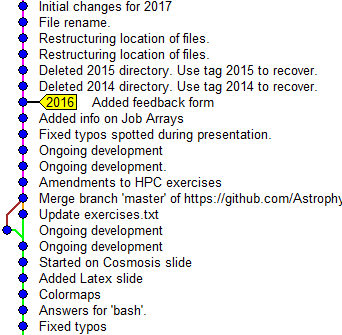
\includegraphics[scale=0.6]{Tag.png}
    \end{center}
  \end{block}
\end{frame}
  
\begin{frame}{Pointers to nodes - branches (1)}
  \begin{block}{}
    \begin{itemize}
      \item{A \textit{branch} is a moveable label that is attached to a node.}
      \item{Here `moveable' means that if you commit an edit to that node then the branch label moves to the child node.}
    \end{itemize}
  \end{block}
  \begin{block}{}
    %\begin{center}
      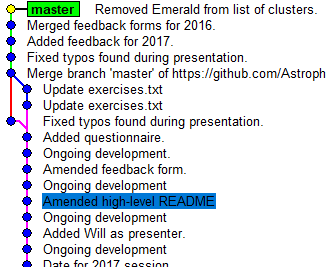
\includegraphics[width=0.5\textwidth]{Branch_1.png}%
      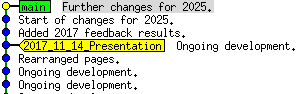
\includegraphics[width=0.5\textwidth]{Branch_2.png}
    %\end{center}
  \end{block}
\end{frame}
  
\begin{frame}{Pointers to nodes - branches (2)}
  \begin{block}{}
    \begin{itemize}
      \item{Because it moves with the commits, the branch is often thought of as a `development line' (imagine not just the node that the branch points to, but also all the past and future nodes that the branch has pointed to or will point to).}
      \item{In some contexts (e.g. cloning) a branch is used to refer not only to the pointed-to node but also all its ancestors.}
    \end{itemize}
  \end{block}
\end{frame}

\begin{frame}{Pointers to nodes - branches (3)}
  \begin{block}{}
    \begin{itemize}
      \item{A branch can point to any node in the DAG - not just to a terminal node (= node with no descendents).}
      \item{So `branch' is not a perfect metaphor; better is `pointer to a place where growth may occur' (which may be on the trunk).}
    \end{itemize}
  \end{block}
  \begin{block}{}
    \begin{center}
      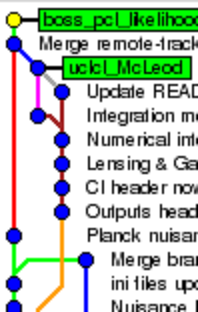
\includegraphics[scale=0.4]{Branch_3.png}
    \end{center}
  \end{block}
\end{frame}

\begin{frame}{Pointers to nodes - branches (4)}
  \begin{block}{}
    \begin{itemize}
      \item{When git creates a new repository it creates a branch called `master' that points to the root node.}
      \item{In the git community `master' is usually taken to mean `the main development line' and house rules often insist that the node pointed to by `master' be `good' (i.e. stable, tested, usable).}
      \item{But this is not forced by git. You don't even need to have a master branch.}
    \end{itemize}
  \end{block}
\end{frame}

\begin{frame}{Pointers to nodes - HEAD (1)}
  \begin{block}{}
    \begin{itemize}
      \item{The special pointer HEAD points to the node that corresponds to the files in the working directory. This can be any node in the DAG.}
      \item{In gitk the HEAD node is shown in yellow.}
    \end{itemize}
  \end{block}
  \begin{block}{}
    \begin{center}
      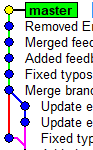
\includegraphics[scale=0.8]{Head.png}
    \end{center}
  \end{block}
\end{frame}

\begin{frame}{Pointers to nodes - HEAD (2) - Detached HEAD}
  \begin{block}{}
    \begin{itemize}
      \item{Usually HEAD points to the same node as one of the branches. But it doesn't have to; if it doesn't then we say we have a `detached HEAD'.}
    \end{itemize}
  \end{block}
  \begin{block}{}
    \begin{center}
      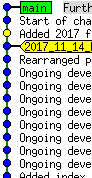
\includegraphics[scale=0.8]{DetachedHead.png}
    \end{center}
  \end{block}
\end{frame}

\begin{frame}{Name that node}
  \begin{block}{}
    \begin{itemize}
      \item{Refer to a node using its (abbreviated) SHA1 name e.g. `c2d2ea34'.}
      \item{Or use a pointer name (a tag name, a branch name, or the name `HEAD').}
      \item{Can append \^{} to mean `parent of', \^{}\^{} to mean `grandparent', etc.}
      \item{Example: \code{git checkout master\^{}\^{}}.}
      \item{Distinguish multiple parents via \^{}1 or \^{}2.}
      \item{Alternatively e.g. \textasciitilde4 means the same as \^{}\^{}\^{}\^{}.}
    \end{itemize}
  \end{block}
\end{frame}

\begin{frame}{DAG manipulation}
  \begin{block}{}
    \begin{itemize}
      \item{Much (but not all) of your interaction with a git repository involves maintaining and amending the DAG and the pointers to nodes in the DAG.}
    \end{itemize}
  \end{block}
\end{frame}


\begin{frame}{The index}
  \begin{block}{}
    \begin{itemize}
      \item{In addition to the DAG, a git repository also contains an \textit{index}: a list of the files in the working directory that git knows about (i.e. that git is `tracking'.}
      \item{The index contains other information that makes it fast to answer the question `has this file changed since a version of it was last put into the repository?'}
    \end{itemize}
  \end{block}
  \begin{block}{}
    \begin{center}
      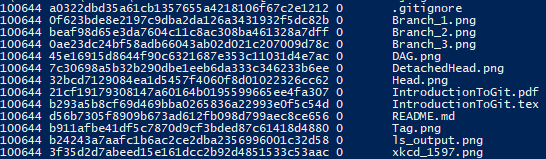
\includegraphics[scale=0.7]{Index.png}
    \end{center}
  \end{block}
\end{frame}

\begin{frame}{.gitignore}
  \begin{block}{}
    \begin{itemize}
      \item{\code{git status} will warn you about files that \textbf{are} in the working directory but \textbf{aren't} in the index (so that git isn't paying attention to them).}
      \item{This gets boring for intermediate files that you never want git to track. So you can list such `files always to be ignored by git' in a special file called .gitignore.}
      \item{So you probably want .gitignore to be one of the files that git is tracking.}
    \end{itemize}
  \end{block}
  \begin{block}{}
    \begin{center}
      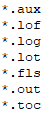
\includegraphics[scale=0.8]{gitignore.png}
    \end{center}
  \end{block}
\end{frame}

\begin{frame}{So three possibilities...}
  \begin{block}{}
    \begin{itemize}
      \item{The index lists the files that git is tracking. (Use \code{git ls-files --stage} to view the index.)}
      \item{The special file .gitignore lists the files that git knows not to track.}
      \item{\code{git status} will warn you about files that are not in either category.}
      \item{Use \code{git add <filename>} to add a file to the index.}
    \end{itemize}
  \end{block}
\end{frame}


\begin{frame}{Three types of git operations}
  \begin{block}{}
    \begin{itemize}
      \item{Managing the relation between a repository and its associated working directory.}
      \item{Repository maintenance.}
      \item{Managing the relation between two repositories (e.g. between your local repository and a copy that is on the Internet).}
    \end{itemize}
  \end{block}
\end{frame}

\begin{frame}{Repository $\leftrightarrow$ working directory (1)}
  \begin{block}{}
    \begin{itemize}
      \item{See a description of the relationship between the repository and the working directory: \code{git status}.}
    \end{itemize}
  \end{block}
  \begin{block}{}
    \begin{center}
      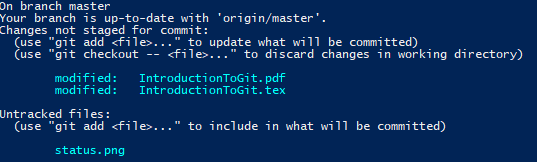
\includegraphics[scale=0.8]{status.png}
    \end{center}
  \end{block}
\end{frame}

\begin{frame}{Repository $\leftrightarrow$ working directory (2)}
  \begin{block}{}
    \begin{itemize}
      \item{Tell the repository's index about a new file in the working directory that you want the repository to pay attention to: \code{git add <filename>}.}
      \item{Check-in the (changed) files that are in the working directory, thereby creating a new node: \code{git commit -a}. TODO: WHAT EXACTLY DEFINES THE PARENT OF THIS NEW NODE?}
      \item{Using the \code{-a} option with \code{commit} minimizes your interaction with the index. There are alternatives that are more work but that give you more control.}
    \end{itemize}
  \end{block}
\end{frame}

\begin{frame}{Repository $\leftrightarrow$ working directory (3)}
  \begin{block}{}
    \begin{itemize}
      \item{Make the working directory be equal to the contents of a specific node: \code{git checkout <nodename>}.}
      \item{This fails if there are uncommited changes in the working directory.}
    \end{itemize}
  \end{block}
\end{frame}

\begin{frame}{Repository maintenance (1)}
  \begin{figure}
    \begin{center}
      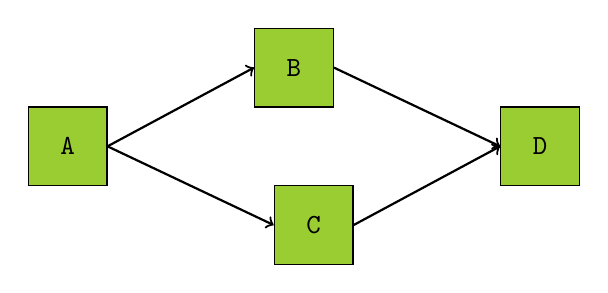
\begin{tikzpicture}[font=\ttfamily]
        \node (A) at (-3,5) [rectangle, draw,minimum height=1cm, minimum width=1cm, align=center, fill=YellowGreen] {A};
        \node (B) at (-0.125,6) [rectangle, draw,minimum height=1cm, minimum width=1cm, align=center, fill=YellowGreen] {B};
        \node (C) at (0.125,4) [rectangle, draw,minimum height=1cm, minimum width=1cm, align=center, fill=YellowGreen] {C};
        \node (D) at (3,5) [rectangle, draw,minimum height=1cm, minimum width=1cm, align=center, fill=YellowGreen] {D};
        \draw [->,thick] (A.east) -- (B.west) node [midway,left] {};
        \draw [->,thick] (A.east) -- (C.west) node [midway,left] {};
        \draw [->,thick] (B.east) -- (D.west) node [midway,left] {};
        \draw [->,thick] (C.east) -- (D.west) node [midway,left] {};
      \end{tikzpicture}
    \end{center}
  \end{figure}
  \begin{block}{}
    \begin{itemize}
      \item{Merge two nodes (here, B and C) to form a new node D with both B and C as its parents.}
    \end{itemize}
  \end{block}
\end{frame}

\begin{frame}{Merging (1)}
  \begin{figure}
    \begin{center}
      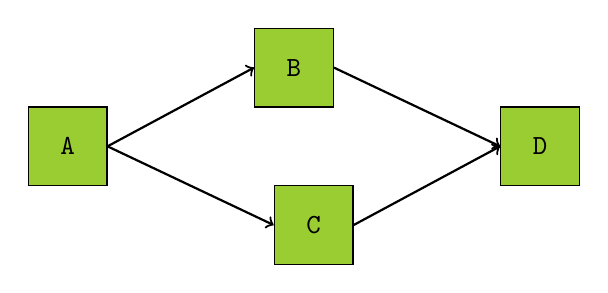
\begin{tikzpicture}[font=\ttfamily]
        \node (A) at (-3,5) [rectangle, draw,minimum height=1cm, minimum width=1cm, align=center, fill=YellowGreen] {A};
        \node (B) at (-0.125,6) [rectangle, draw,minimum height=1cm, minimum width=1cm, align=center, fill=YellowGreen] {B};
        \node (C) at (0.125,4) [rectangle, draw,minimum height=1cm, minimum width=1cm, align=center, fill=YellowGreen] {C};
        \node (D) at (3,5) [rectangle, draw,minimum height=1cm, minimum width=1cm, align=center, fill=YellowGreen] {D};
        \draw [->,thick] (A.east) -- (B.west) node [midway,left] {};
        \draw [->,thick] (A.east) -- (C.west) node [midway,left] {};
        \draw [->,thick] (B.east) -- (D.west) node [midway,left] {};
        \draw [->,thick] (C.east) -- (D.west) node [midway,left] {};
      \end{tikzpicture}
    \end{center}
  \end{figure}
  \begin{block}{}
    \begin{itemize}
      \item{Merging requires B and C to have a common ancestor (A in the above example). In git this will always be the case.}
      \item{Form the union of the `A to B' changes and the `A to C' changes. Then apply these united changes to A; this gives D.}
    \end{itemize}
  \end{block}
\end{frame}

\begin{frame}{Merging (2)}
  \begin{block}{}
    \begin{itemize}
      \item{`Changes' include: adding files, deleting files, and amending files (by adding lines, deleting lines, or amending lines).}
      \item{Perhaps the `A to B' changes and the `A to C' changes are in conflict. For example, both sets of changes might amend a certain line, but in different ways.}
      \item{In this case the merge will fail, and you will have to manually edit D to choose one set of changes or the other (they will both be present in D, with special characters inserted to let you see what is going on).}
      \item{At merge time the `level of granularity' is the line (if I amend the start of a line and you amend the end of the same line, then the merge will still fail.) Note that binary files can't be merged.}
    \end{itemize}
  \end{block}
\end{frame}

\begin{frame}{Rebase (1)}
  \begin{block}{}
    \begin{itemize}
      \item{\textit{Rebase} is similar to merge, in that it allows two separate development streams to be brought together.}
      \item {However, the mental picture with rebase is `move the A to C arrow so that it starts from B instead of from A'.}
      \item {Alternatively can think of this as being a `cut and paste' to move part of the DAG from one place to another.}
    \end{itemize}
  \end{block}
\end{frame}

\begin{frame}{Rebase (2)}
  \begin{figure}
    \begin{center}
      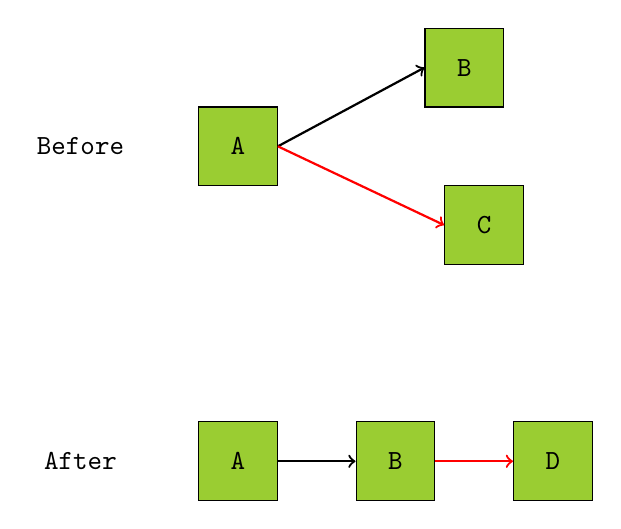
\begin{tikzpicture}[font=\ttfamily]
        \node[] at (-5,5) {Before};
        \node (A) at (-3,5) [rectangle, draw,minimum height=1cm, minimum width=1cm, align=center, fill=YellowGreen] {A};
        \node (B) at (-0.125,6) [rectangle, draw,minimum height=1cm, minimum width=1cm, align=center, fill=YellowGreen] {B};
        \node (C) at (0.125,4) [rectangle, draw,minimum height=1cm, minimum width=1cm, align=center, fill=YellowGreen] {C};
        \draw [->,thick] (A.east) -- (B.west) node [midway,left] {};
        \draw [->,thick,red] (A.east) -- (C.west) node [midway,left] {};

        \node[] at (-5,1) {After};
        \node (A1) at (-3,1) [rectangle, draw,minimum height=1cm, minimum width=1cm, align=center, fill=YellowGreen] {A};
        \node (B1) at (-1,1) [rectangle, draw,minimum height=1cm, minimum width=1cm, align=center, fill=YellowGreen] {B};
        \node (D) at (1,1) [rectangle, draw,minimum height=1cm, minimum width=1cm, align=center, fill=YellowGreen] {D};
        \draw [->,thick] (A1.east) -- (B1.west) node [midway,left] {};
        \draw [->,thick,red] (B1.east) -- (D.west) node [midway,left] {};
      \end{tikzpicture}
    \end{center}
  \end{figure}
\end{frame}

\begin{frame}{Cherry-pick (1)}
  \begin{block}{}
    \begin{itemize}
      \item{\textit{Cherry-pick} is similar to rebase, except that it is a `copy and paste' instead of a `cut and paste'.}
    \end{itemize}
  \end{block}
\end{frame}

\begin{frame}{Cherry-pick (2)}
  \begin{figure}
    \begin{center}
      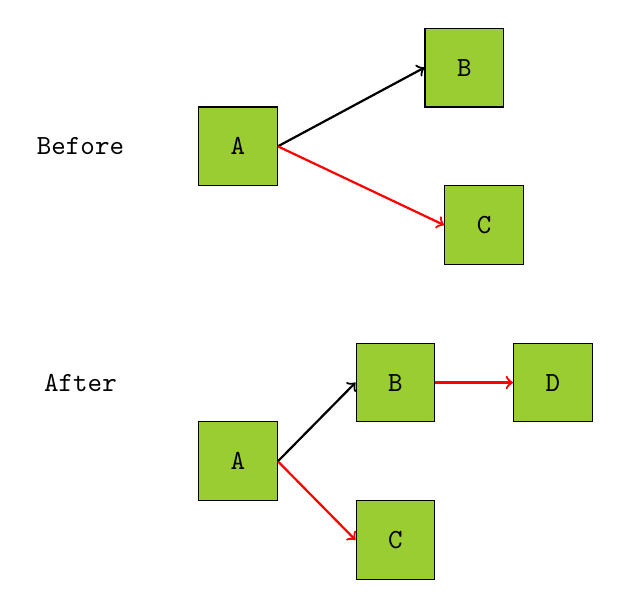
\begin{tikzpicture}[font=\ttfamily]
        \node[] at (-5,5) {Before};
        \node (A) at (-3,5) [rectangle, draw,minimum height=1cm, minimum width=1cm, align=center, fill=YellowGreen] {A};
        \node (B) at (-0.125,6) [rectangle, draw,minimum height=1cm, minimum width=1cm, align=center, fill=YellowGreen] {B};
        \node (C) at (0.125,4) [rectangle, draw,minimum height=1cm, minimum width=1cm, align=center, fill=YellowGreen] {C};
        \draw [->,thick] (A.east) -- (B.west) node [midway,left] {};
        \draw [->,thick,red] (A.east) -- (C.west) node [midway,left] {};

        \node[] at (-5,2) {After};
        \node (A1) at (-3,1) [rectangle, draw,minimum height=1cm, minimum width=1cm, align=center, fill=YellowGreen] {A};
        \node (B1) at (-1,2) [rectangle, draw,minimum height=1cm, minimum width=1cm, align=center, fill=YellowGreen] {B};
        \node (C1) at (-1,0) [rectangle, draw,minimum height=1cm, minimum width=1cm, align=center, fill=YellowGreen] {C};
        \node (D) at (1,2) [rectangle, draw,minimum height=1cm, minimum width=1cm, align=center, fill=YellowGreen] {D};
        \draw [->,thick,red] (A1.east) -- (C1.west) node [midway,left] {};
        \draw [->,thick] (A1.east) -- (B1.west) node [midway,left] {};
        \draw [->,thick,red] (B1.east) -- (D.west) node [midway,left] {};
      \end{tikzpicture}
    \end{center}
  \end{figure}
\end{frame}

\begin{frame}{Pointer maintenance}
  \begin{block}{}
    \begin{itemize}
      \item{Tags and branches can be created, moved and deleted.}
      \item{Recall that a branch is just a pointer to a node. So moving a branch doesn't involve any rearrangement of the DAG - it means simply changing the node to which the branch points.}
    \end{itemize}
  \end{block}
\end{frame}

\begin{frame}{Node cleanup}
  \begin{block}{}
    \begin{itemize}
      \item{If a node is not `named' (i.e. pointed to by a tag or a branch), and if none of its descendents are named either, then git considers it unneeded and will delete it the next time it does `automatic cleanup'.}
      \item{Recall that a branch is just a pointer to a node. So moving a branch doesn't involve any rearrangement of the DAG - it means simply changing the node to which the branch points.}
    \end{itemize}
  \end{block}
\end{frame}



\end{document}
